\subsection{Introducción}

El problema que querremos resolver en este caso, es la separación de clusters, en donde se nos dan un conjunto de puntos en un plano de dos dimensiones y querremos agrupar en distintos clusters los puntos que estan más juntos. Se puede obsrevar a simple vista que este problema no tiene un resultado exacto, ya que decir que un conjunto de puntos se encuentran mas juntos que otro onjunto de puntos es totalmente subjetivo a la persona que los observe. 




\subsection{Desarrollo}

En primer lugar generaremos un grafo completo, en donde los puntos serán los vertices, y el peso de los ejes es la distancia euclidea entre los vertices que conecta. Luego el problema pasa a ser un problema de generar componentes conexas, donde se debe cumplir que todos los vertices pertenecientes a una misma componente se encuentran cerca a comparación con los vertices de las otras componentes.

Zahn nos recomienda en su paper que generemos el Árbol Generador Mínimo (AGM), asi de esta manera, generar un componente es simplemente quitar un eje, por definición de árbol. No solo eso, sino que además al ser el AGM y no cualquier otro Árbol Generador, obligará a que los vertices esten conectados con los vertices mas cercános (sin generar ciclos), que es lo que queremos obtener, ya que es diferenciar los puntos cercanos entre otros puntos lejanos.


\begin{figure}[H]
  \begin{center}
    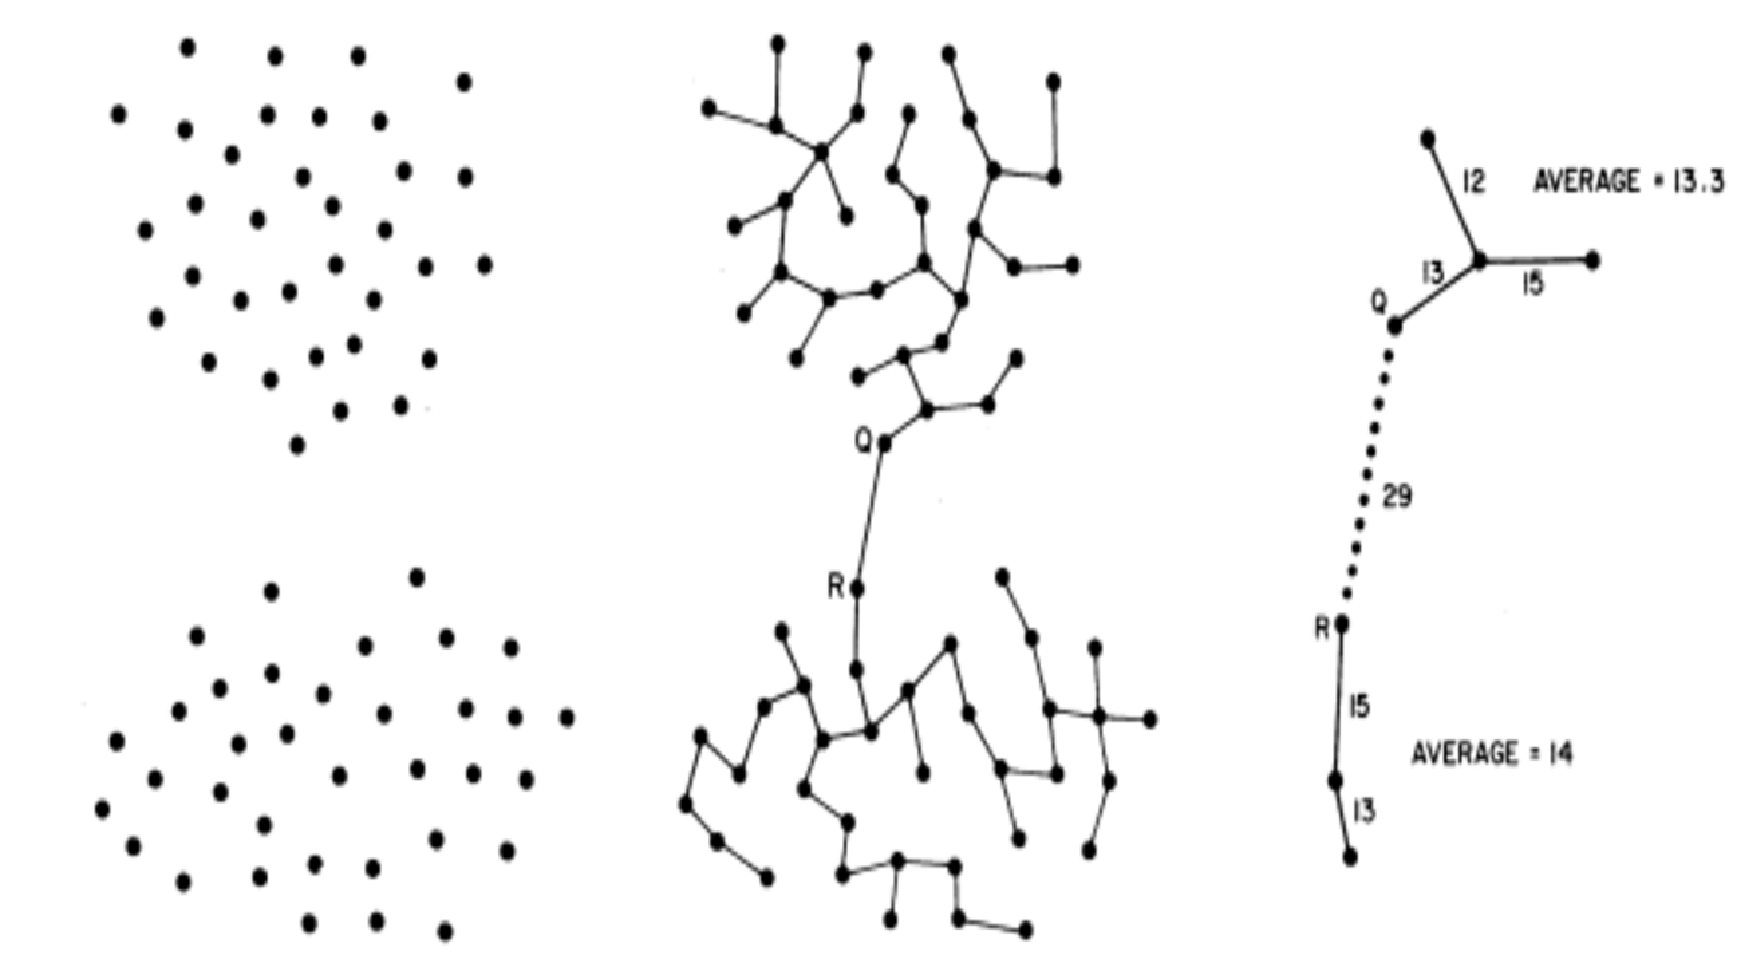
\includegraphics[scale=0.45]{img/agm_demo.pdf}
    \caption{Ejemplo de quitado de un eje}
    \label{arbol_muestra}
  \end{center}
\end{figure}



Al observar la Figura \ref{arbol_muestra}, podemos observar que en definitiva al obtener el AGM del grafo, se obtiene que los vertices se conectan con aquellos vertices mas cercanos, exceptuando un eje que conecta los "cluster". Este eje es el que define Zahn como eje inconsistente y los describe como aquel que cumple alguna de las siguientes propiedades:

\begin{itemize}
    \item El promedio del peso de la vecindad"ref" de cada nodo es menor que el peso del eje que los une.
    \item El desvio estandar del peso de la vecindad"ref" de cada nodo es menor que el peso del eje que los une.
\end{itemize}

    